\documentclass[11pt,a4paper]{article}
\usepackage[utf8]{inputenc}\usepackage[T1]{fontenc}\usepackage[brazilian]{babel}
\usepackage[margin=2cm]{geometry}\usepackage{graphicx,booktabs,longtable,amsmath,amssymb,hyperref,float,xcolor,fancyhdr}
\definecolor{ink}{HTML}{203448}\definecolor{accent}{HTML}{087F8C}
\hypersetup{colorlinks=true,urlcolor=accent,linkcolor=ink,pdftitle={Previsão temporal de traços: GRU versus MLP DeepSets},pdfauthor={Pedro Martineli}}
\setlength{\parindent}{0pt}\setlength{\parskip}{6pt}\setlength{\headheight}{14pt}
\pagestyle{fancy}\fancyhf{}\fancyhead[L]{\small Projeto 4 — Previsão de séries temporais}\fancyhead[R]{\small Quick, Draw!}\fancyfoot[C]{\thepage}
\begin{document}\begin{center}{\Large\bfseries\color{ink} Previsão temporal de traços: GRU versus MLP DeepSets}\\[5pt]
Introdução às Redes Neurais Artificiais\\Pedro Martineli (RA: 193474)
\end{center}\textbf{Resumo.} Este trabalho prevê os próximos eventos da caneta em desenhos do Quick, Draw!, usando uma rede recorrente GRU como modelo principal e um MLP DeepSets como comparação sem recorrência. A avaliação mantém dados, categoria fornecida, banco de trajetórias, decoder, perdas e orçamento comuns. A busca utiliza somente a validação, com treinamento do zero e três réplicas da configuração escolhida. Em 30 eventos futuros, o ADE médio foi 138,6 pixels para a GRU e 161,2 para o MLP. O relatório analisa horizontes, quantidade de contexto, cruzamentos, estado da caneta, tempo, ordem e transformações geométricas, acompanhados de exemplos visuais. As conclusões distinguem propriedades da representação de evidências específicas da recorrência. O teste é uma partição já explorada em estudos anteriores, não uma validação externa inédita.
\section{Problema de previsão e planejamento experimental}
O objetivo é receber uma janela de eventos observados até t e prever as posições da caneta, os estados de desenho e os intervalos dos próximos k eventos. O trabalho concentra-se exclusivamente em previsão de séries temporais. A categoria é uma condição fornecida, e não uma saída de reconhecimento. Usamos uma GRU para representar a evolução do estado e um MLP DeepSets para representar o conjunto dos eventos, com o mesmo decoder nos dois casos. A comparação procura identificar quando a ordem sequencial contribui para a continuação, sem pressupor superioridade universal da RNN.
\subsection{Busca de hiperparâmetros e escolha pela validação}
Cada família compara larguras 128/192 e taxas iniciais 0,001/0,0005. Todos os modelos foram construídos do zero: nenhuma rede é inicializada com os pesos de outra. O banco de 64 modos por categoria é ajustado apenas no treino e compartilhado. Os quatro treinos GRU da triagem, já executados com este protocolo, são reutilizados como execuções completas com hashes e proveniência; isso não constitui transferência para inicializar o MLP. A triagem usa seed 42. Dois finalistas por família são treinados novamente com seed 43; arquitetura e limiar de pen-up comuns minimizam a média de validação nas seeds 42/43. A réplica 44 é posterior à decisão. Nenhum resultado de teste escolhe uma configuração desta comparação.
\begingroup\small\setlength{\tabcolsep}{4pt}\begin{longtable}{lrrrrr}
\caption{Triagem seed42 por família; menor J é melhor.}\\
\toprule
Rede & Unidades & LR inicial & Época & Limiar & J val. \\ 
\midrule\endfirsthead
\toprule
Rede & Unidades & LR inicial & Época & Limiar & J val. \\ 
\midrule\endhead
\bottomrule\endfoot
GRU & 128 & 0,0010 & 17 & 0,20 & 0,396 \\
GRU & 128 & 0,0005 & 20 & 0,20 & 0,420 \\
GRU & 192 & 0,0010 & 18 & 0,20 & 0,380 \\
GRU & 192 & 0,0005 & 17 & 0,20 & 0,405 \\
MLP DeepSets & 128 & 0,0010 & 16 & 0,20 & 0,446 \\
MLP DeepSets & 128 & 0,0005 & 16 & 0,20 & 0,454 \\
MLP DeepSets & 192 & 0,0010 & 16 & 0,20 & 0,440 \\
MLP DeepSets & 192 & 0,0005 & 18 & 0,20 & 0,451 \\
\end{longtable}\endgroup
\begingroup\small\setlength{\tabcolsep}{4pt}\begin{longtable}{lrrrrrr}
\caption{Decisão entre finalistas, com limiar compartilhado entre seeds.}\\
\toprule
Rede & Unidades & LR inicial & Limiar & J42 & J43 & Média \\ 
\midrule\endfirsthead
\toprule
Rede & Unidades & LR inicial & Limiar & J42 & J43 & Média \\ 
\midrule\endhead
\bottomrule\endfoot
GRU & 192 & 0,0010 & 0,20 & 0,380 & 0,380 & 0,380 \\
GRU & 128 & 0,0010 & 0,20 & 0,396 & 0,391 & 0,394 \\
MLP DeepSets & 192 & 0,0010 & 0,20 & 0,440 & 0,438 & 0,439 \\
MLP DeepSets & 128 & 0,0010 & 0,20 & 0,446 & 0,445 & 0,446 \\
\end{longtable}\endgroup
\begin{figure}[H]\centering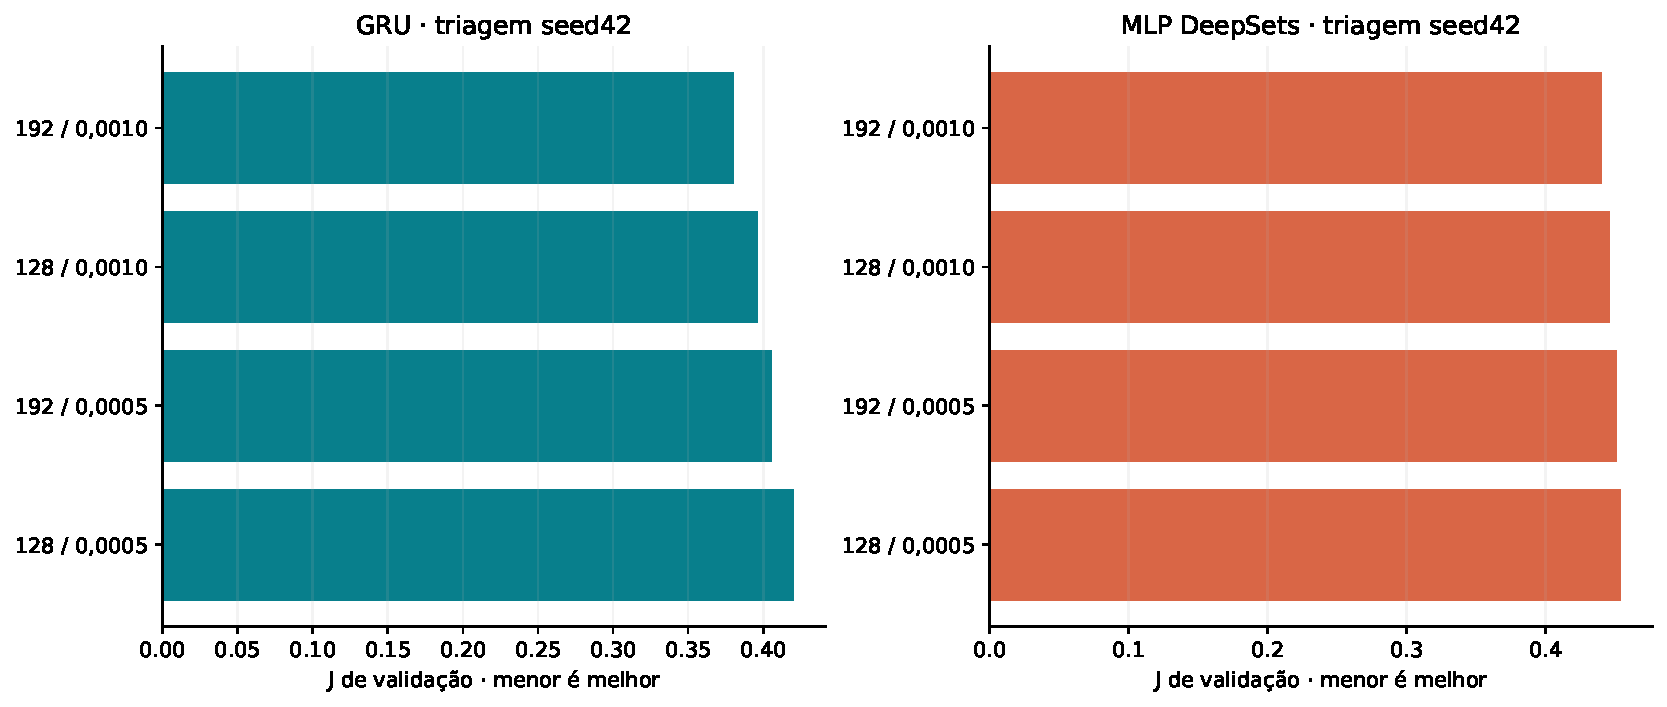
\includegraphics[width=\linewidth,height=.58\textheight,keepaspectratio]{../figures/c_busca.pdf}\caption{Busca na validação. As duas famílias utilizam o mesmo critério, alvos e orçamento.}\end{figure}
\subsection{Critério, taxas e orçamento de treinamento}
O orçamento comum é de 20 épocas, lote 128, AdamW, weight decay 0,00001, clipping da norma do gradiente em 1 e taxa cossenoidal até 10\% da inicial. A augmentação isotrópica de escala 0,8–1,2 ocorre somente no treino e é a mesma nas duas famílias. O checkpoint de cada execução minimiza a média de ADE/256 + 0,1 vezes a frequência de fim precoce nos horizontes 5/15/30, nos primeiros 100 desenhos de validação por classe. A seleção externa usa toda a validação, acrescenta a penalidade de F1 de pen-up e testa limiares 0,2/0,35/0,5. A perda supervisionada combina CE do modo, 8$\times$Huber de posição, 0,4$\times$Huber de deslocamentos, CE da caneta, 0,15$\times$Huber do relógio e 0,2$\times$suavidade das correções. Nenhum ponto real futuro é fornecido na inferência da validação.
\[
J=\frac{1}{3}\sum_{k\in\{5,15,30\}}\left[\frac{\mathrm{ADE}_k}{256}+0{,}1\,E_k+0{,}02(1-F1_{\mathrm{pen},k})\right].
\]
\subsection{Curvas de aprendizagem e capacidade}
As curvas distinguem a perda composta do treino e o critério de trajetória usado na validação. Como possuem definições e unidades diferentes, seus valores não devem ser subtraídos como um gap direto. As estrelas indicam o melhor checkpoint de cada seed. O número de parâmetros é informado porque igual largura oculta não implica igual capacidade entre GRU e MLP. O tempo mostrado é o observado na execução seed42 da rede escolhida, na RTX 4050 de 6 GB em float32, com determinismo habilitado; não é um benchmark controlado de energia ou latência. A cabeça de correções começa zerada nos dois modelos; as demais camadas utilizam inicialização por seed.
\begingroup\small\setlength{\tabcolsep}{4pt}\begin{longtable}{lrrrrr}
\caption{Configurações finais e custo observado; tempo em segundos.}\\
\toprule
Rede & Unidades & LR inicial & Parâmetros & Época42 & Tempo42 \\ 
\midrule\endfirsthead
\toprule
Rede & Unidades & LR inicial & Parâmetros & Época42 & Tempo42 \\ 
\midrule\endhead
\bottomrule\endfoot
GRU & 192 & 0,0010 & 189.492 & 18 & 53,4 \\
MLP DeepSets & 192 & 0,0010 & 143.796 & 16 & 42,4 \\
\end{longtable}\endgroup
\begin{figure}[H]\centering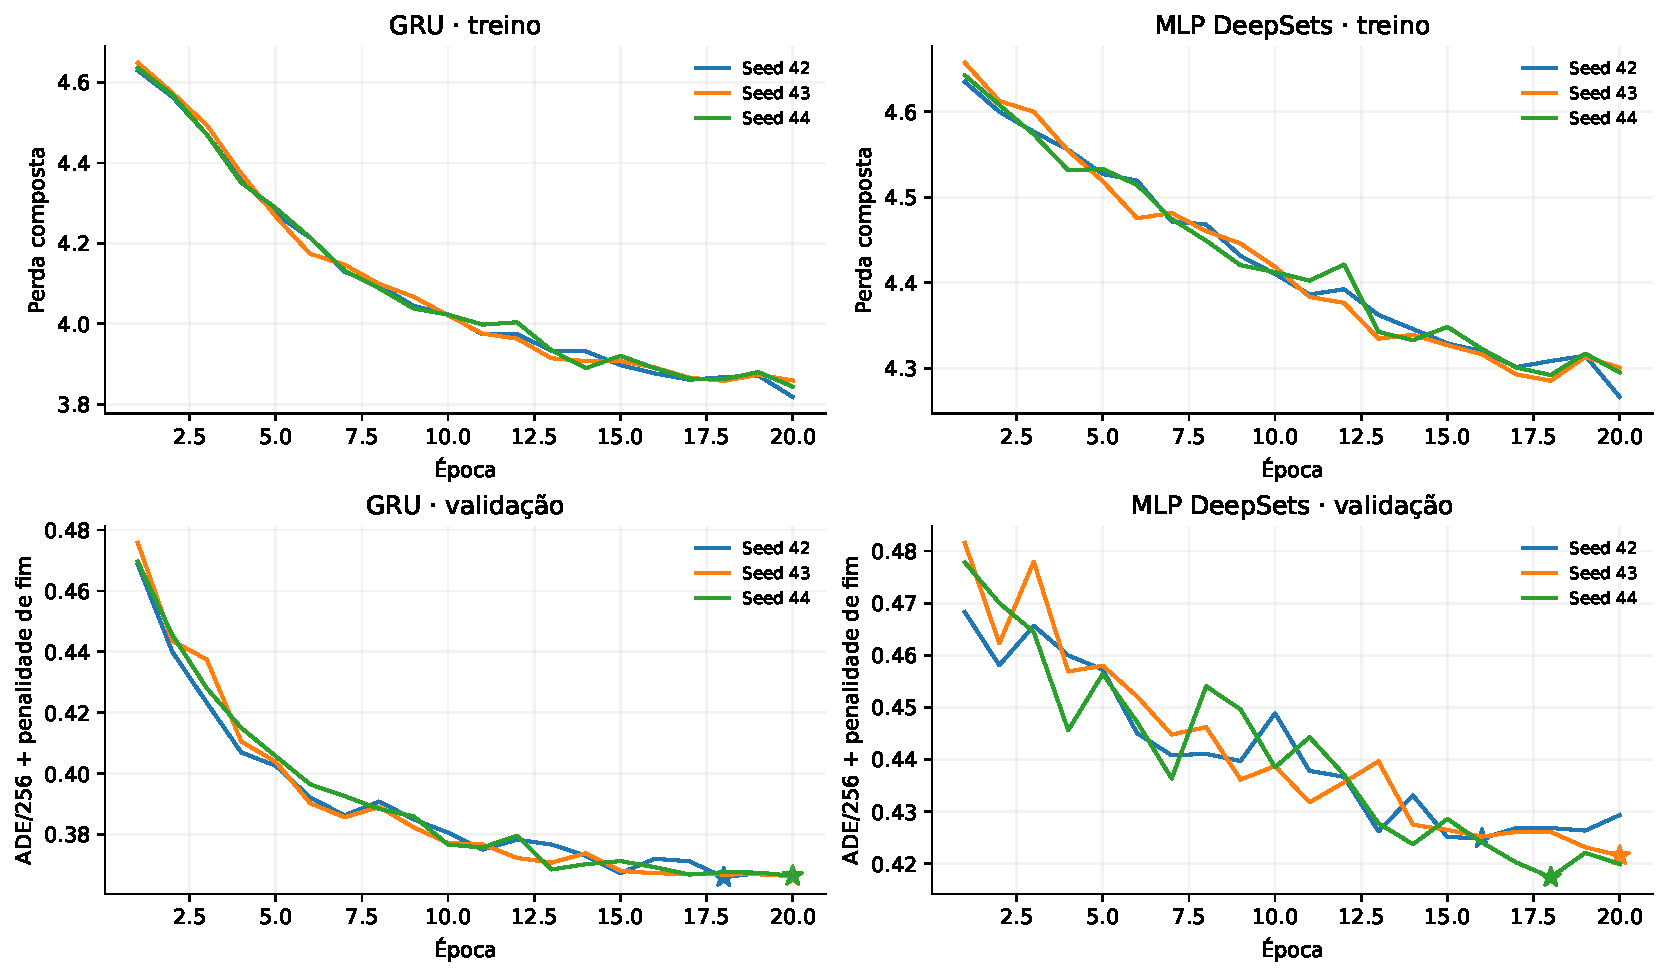
\includegraphics[width=\linewidth,height=.58\textheight,keepaspectratio]{../figures/d_aprendizagem.pdf}\caption{Aprendizagem das três réplicas de cada família. Checkpoints são escolhidos pela validação.}\end{figure}
\section{Dados, representação temporal e saídas}
Utilizamos 42 mil desenhos de 12 categorias: gato, peixe, flor, casa, árvore, guarda-chuva, cachorro, tubarão, castelo, cacto, carro e bicicleta. São 36 mil de treino, 3 mil de validação e 3 mil de teste, balanceados por categoria e com desenhos inteiros em uma única partição. O recorte inclui somente desenhos reconhecidos pelo jogo original. Os mesmos IDs e geometrias ficam congelados para ambas as famílias. As partições já foram usadas anteriormente; a comparação é interna sobre esse teste. Não há separação garantida por autor. Os arquivos preparados, seus hashes e os manifests permitem reconstruir o recorte sem depender de outros experimentos.
\subsection{O que entra na rede}
O dado bruto contém traços com X, Y e tempos em milissegundos. Derivamos o estado de caneta a partir dos limites dos traços e convertemos o relógio para segundos relativos ao primeiro ponto. A amostragem causal mantém pontos após 14 pixels de deslocamento já observado, preservando fronteiras e tempos. Filtramos 12–180 eventos, até 4 mil pontos brutos e duração positiva até 60 s. Cada evento é um vetor de seis valores. O desvio dos deslocamentos, 28,80 pixels, é calculado só no treino; posições usam escala fixa 256 e tempo 0,1 s. A categoria vira um embedding de 16 dimensões concatenado a cada evento: o encoder recebe 22 atributos por passo. O contexto contém no máximo 64 eventos; comprimentos e máscaras excluem preenchimento.
\[
\mathbf u_i=\left[\frac{\Delta x_i}{s_\Delta},\frac{\Delta y_i}{s_\Delta},p_i,\log\left(1+\frac{\Delta\tau_i}{0{,}1\,\mathrm{s}}\right),\frac{x_i-x_0}{256},\frac{y_i-y_0}{256}\right].
\]
\begingroup\small\setlength{\tabcolsep}{4pt}\begin{longtable}{lrr}
\caption{Entrada e alvo na tarefa de previsão.}\\
\toprule
Elemento & Formato & Conteúdo \\ 
\midrule\endfirsthead
\toprule
Elemento & Formato & Conteúdo \\ 
\midrule\endhead
\bottomrule\endfoot
Prefixo & B $\times$ w $\times$ 6 & Eventos observados, w $\leq$64 \\
Categoria & B índices & Condição conhecida, 12 categorias \\
Entrada ao encoder & B $\times$ w $\times$ 22 & Evento e embedding \\
Alvos futuros & B $\times$ k eventos & X/Y, caneta e tempo reais \\
Saída interpretável & B $\times$ k $\times$ 4 & X/Y, estado e intervalo previstos \\
\end{longtable}\endgroup
\begin{figure}[H]\centering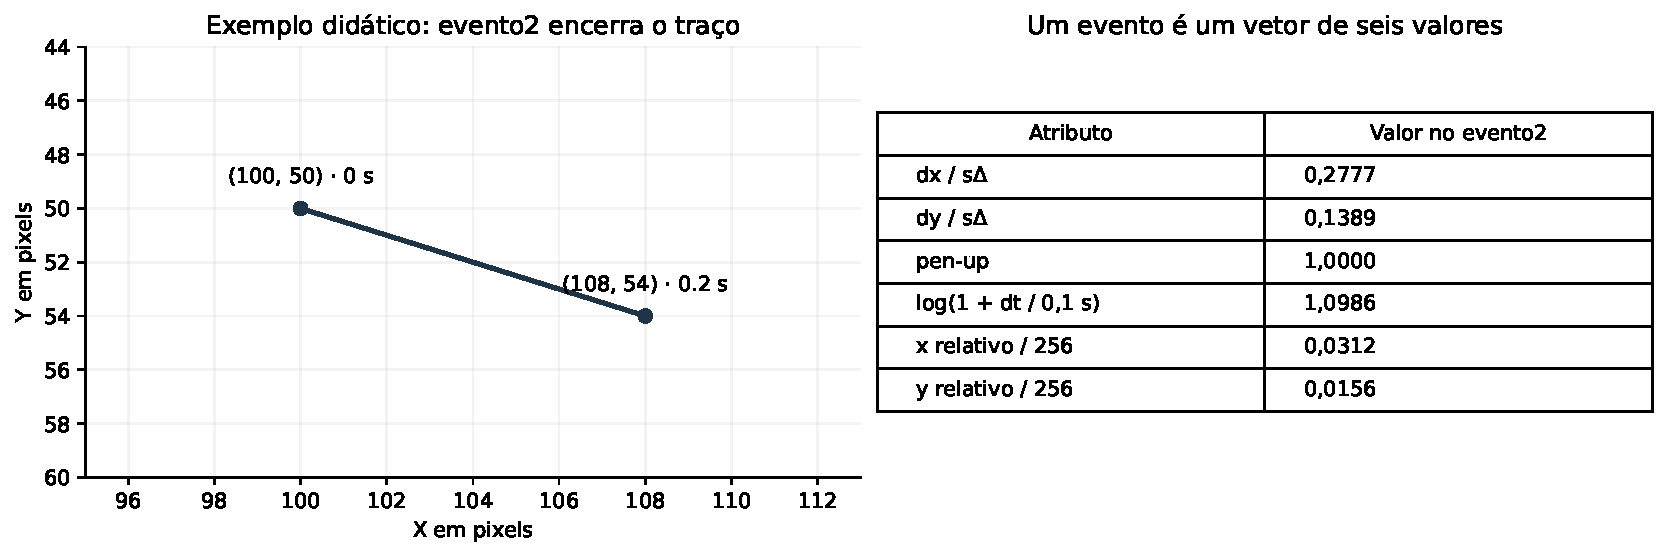
\includegraphics[width=\linewidth,height=.58\textheight,keepaspectratio]{../figures/b_entrada_eventos.pdf}\caption{Exemplo didático de codificação, não uma previsão selecionada pelo acerto. O primeiro movimento e o primeiro intervalo são zero.}\end{figure}
\subsection{O que significa prever t+k}
t é um índice de evento, não um instante uniformemente espaçado em segundos. Se 32 eventos foram observados, k=5 prevê os eventos 33–37, enquanto k=30 prevê 33–62. Os intervalos entre esses eventos também são previstos. A saída interna do decoder tem seis valores por evento: duas coordenadas, três escores de estado e um valor de relógio. A saída decodificada é X, Y, estado e intervalo; o código também conserva deslocamentos e uma máscara de encerramento. Depois de encerrar, a posição é mantida, a caneta fica levantada e o relógio não avança. Encerrar enquanto ainda há futuro real é contado como erro, não como remoção da amostra.
\[
\widehat{\mathbf S}_{t+1:t+k}=f_\theta(\mathbf u_{t-w+1:t},c),\quad k\in\{5,15,30\},\quad\widehat\tau_{t+j}=\tau_t+\sum_{\ell=1}^j\widehat{\Delta\tau}_{t+\ell}.
\]
\section{Como isolamos a contribuição da recorrência}
A GRU atualiza um estado h a cada evento. O DeepSets aplica um MLP Tanh 22$\to$H$\to$H a cada evento, calcula uma média mascarada, concatena a contagem observada w/64 e usa uma camada de fusão para produzir um estado do mesmo tamanho. Esse encoder não possui GRU, LSTM ou outra recorrência. A média é invariável a permutações dos vetores, mas os próprios vetores já contêm movimento e tempo locais. Além disso, o decoder comum usa o último ponto e a direção dos últimos movimentos observados. Portanto, não se deve chamar o MLP inteiro de totalmente cego à ordem ou invariável a qualquer permutação da entrada. O ramo visual CNN de estudos anteriores não integra esta comparação principal.
\[
h_i^{\mathrm{GRU}}=\operatorname{GRU}([\mathbf u_i,e(c)],h_{i-1}),
\]
\[
h^{\mathrm{MLP}}=\tanh\!\left(W_\rho\left[\frac{\sum_i m_i\phi([\mathbf u_i,e(c)])}{\sum_i m_i},\frac{\sum_i m_i}{64}\right]+b_\rho\right).
\]
\begin{figure}[H]\centering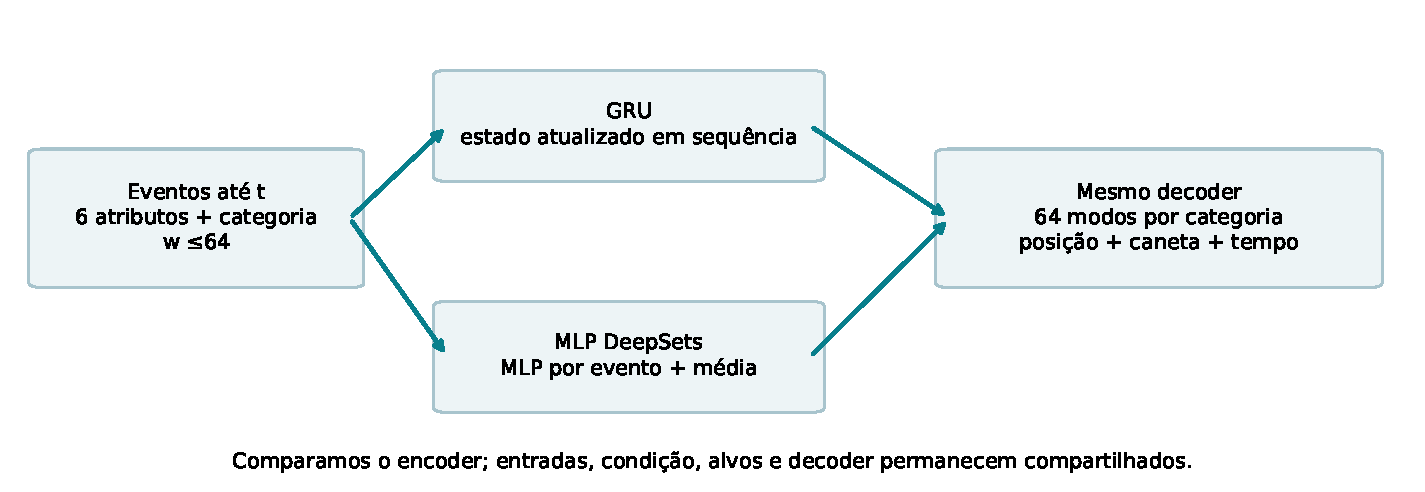
\includegraphics[width=\linewidth,height=.58\textheight,keepaspectratio]{../figures/a_arquiteturas.pdf}\caption{Comparação dos encoders, com condição e decoder compartilhados. A RNN é o modelo principal; o MLP é um controle arquitetural concreto, não qualquer rede possível.}\end{figure}
\subsection{Decoder compartilhado e hipóteses de trajetória}
O banco contém 64 padrões de 30 eventos por categoria, aprendido com três janelas de cada desenho de treino. A seleção supervisionada do modo usa o futuro somente como alvo da perda durante o treino. Na inferência, o modo vem apenas do passado e da categoria fornecida. A rede prevê correções limitadas por tanh e estados de caneta e relógio. O referencial usa a última posição e a direção dos últimos três segmentos válidos de tinta, sem coordenadas futuras. Não há busca por desenhos parecidos na inferência. Compartilhar esse mecanismo controla uma parte importante da representação, mas também limita a diversidade das duas famílias. A inspiração em modos vem de MultiPath; a implementação não reproduz o artigo nem o Sketch-RNN.
\section{Hipóteses sobre o que a RNN pode ajudar}
Ideias intuitivas sobre memória precisam ser transformadas em perguntas mensuráveis. As redes usadas aqui são GRUs, não LSTMs. Frases sobre reconhecer maçã ou sol, separar perfeitamente partes de objetos ou ser imune a rabiscos não são resultados deste estudo. As categorias citadas nesses exemplos nem fazem parte do recorte de 12 classes. O que medimos é a continuação condicionada a uma categoria fornecida. As hipóteses abaixo orientam gráficos e controles, sem converter vantagens possíveis em garantias.
\begingroup\small\setlength{\tabcolsep}{4pt}\begin{longtable}{p{.22\linewidth}p{.34\linewidth}p{.34\linewidth}}
\caption{Da intuição ao experimento de previsão.}\\
\toprule
Ideia & Operação no estudo & Limite da conclusão \\ 
\midrule\endfirsthead
\toprule
Ideia & Operação no estudo & Limite da conclusão \\ 
\midrule\endhead
\bottomrule\endfoot
Formas ambíguas & Prever continuações, categoria fornecida & Não mede reconhecimento de sol ou maçã \\
Traços sobrepostos & Erro condicionado a cruzamentos & Não demonstra imunidade nem compara CNN \\
Mais observações & Prefixos e janela com origem fixa & Alvos/coortes e distribuição podem mudar \\
Tamanho e posição & Translação e fatores de escala & $\Delta$ remove translação, não magnitude \\
Caneta levantada & Condicionais e retirada do canal & Retirada sem retreino é sensibilidade OOD \\
\end{longtable}\endgroup
\section{Resultados de teste por horizonte}
Cada previsão recebe apenas o prefixo real, e toda a trajetória futura é emitida sem receber novos pontos reais. Usam-se cortes de 16/32 eventos no resultado principal; o recorte inicial exclui prefixos com cinco ou menos eventos restantes e cada k exige ao menos k eventos futuros. As populações de horizontes diferentes não são idênticas. ADE é a distância euclidiana média ao longo dos k eventos, e FDE é a distância no último evento. O RMSE é calculado por janela nas k$\times$2 coordenadas e depois promediado. A tabela usa médias de três seeds, sem ensemble. Todas as famílias e referências simples usam os mesmos alvos em cada comparação.
\[
\mathrm{ADE}_k=\frac1k\sum_{j=1}^k\|\widehat{\mathbf p}_{t+j}-\mathbf p_{t+j}\|_2,\qquad\mathrm{FDE}_k=\|\widehat{\mathbf p}_{t+k}-\mathbf p_{t+k}\|_2.
\]
\begingroup\small\setlength{\tabcolsep}{4pt}\begin{longtable}{lrrrrrr}
\caption{Médias de teste entre seeds42/43/44; erros em pixels.}\\
\toprule
k & Rede & Prefixos & ADE & FDE & RMSE & DP ADE \\ 
\midrule\endfirsthead
\toprule
k & Rede & Prefixos & ADE & FDE & RMSE & DP ADE \\ 
\midrule\endhead
\bottomrule\endfoot
5 & GRU & 5.914 & 44,7 & 71,3 & 35,8 & 0,23 \\
5 & MLP DeepSets & 5.914 & 50,0 & 81,4 & 40,1 & 0,03 \\
15 & GRU & 5.771 & 94,8 & 149,2 & 77,0 & 0,32 \\
15 & MLP DeepSets & 5.771 & 110,5 & 175,8 & 89,3 & 0,45 \\
30 & GRU & 5.236 & 138,6 & 196,5 & 111,7 & 0,46 \\
30 & MLP DeepSets & 5.236 & 161,2 & 228,4 & 129,0 & 0,33 \\
\end{longtable}\endgroup
\begin{figure}[H]\centering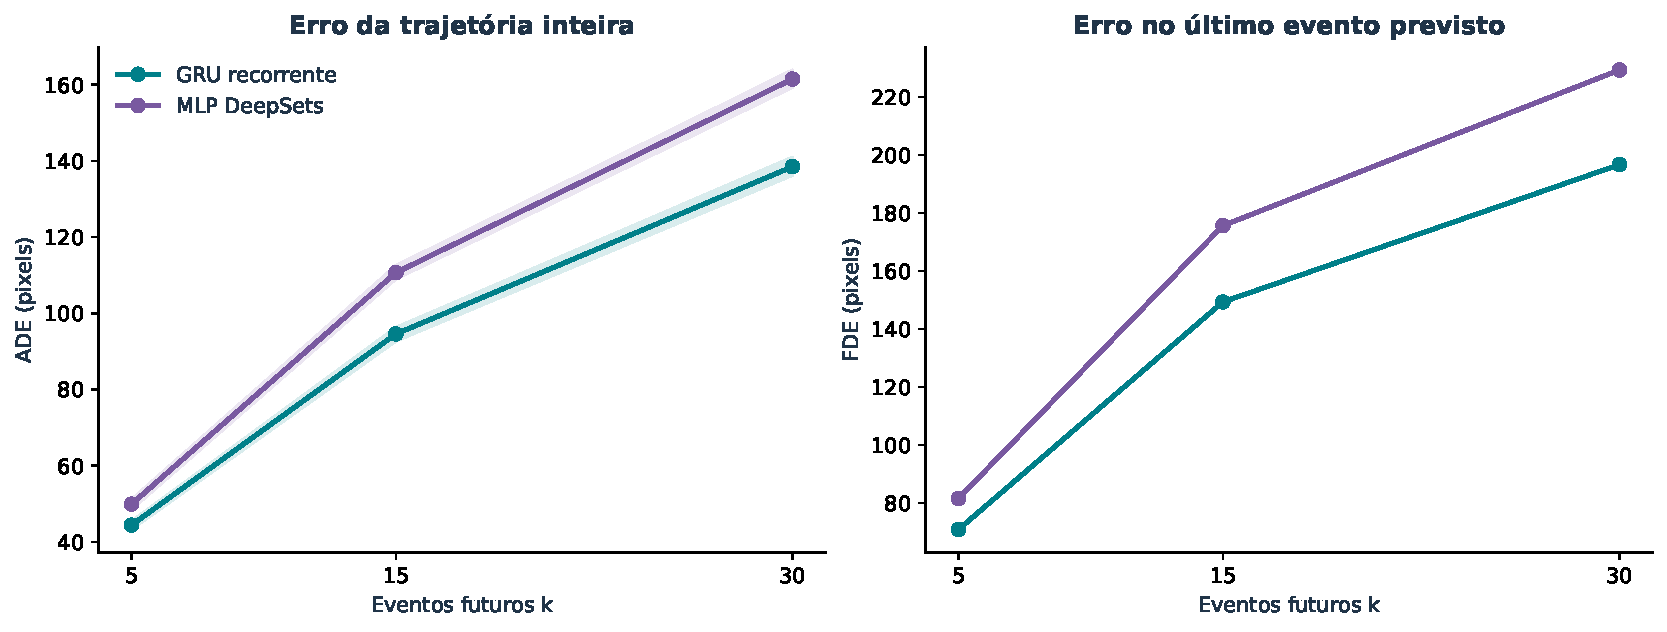
\includegraphics[width=\linewidth,height=.58\textheight,keepaspectratio]{../figures/01_horizons_comparison.pdf}\caption{Mesmos desenhos, cortes16/32 e horizontes em ambas as redes, execução42. ADE mede a trajetória inteira; FDE mede o último ponto. Faixas de95\% do ADE reamostram IDs de desenhos, mantendo seus prefixos juntos.}\end{figure}
\subsection{Réplicas, diferenças pareadas e caudas de erro}
A GRU obteve ADE menor que o MLP nos horizontes 5, 15, 30 eventos. Em 30 eventos, a redução relativa de ADE diante do MLP foi 14,0\%; valores negativos indicam vantagem do comparador. A tabela de réplicas mostra a sensibilidade ao treinamento. Os diagnósticos de caudas e condicionais usam a seed42, definida antes de consultar esses resultados. Os intervalos pareados reamostram desenhos inteiros, preservando juntos seus prefixos. Diferença negativa favorece a GRU. São intervalos condicionais aos pesos, e não intervalos de previsão para um novo traço.
\begingroup\small\setlength{\tabcolsep}{4pt}\begin{longtable}{lrrrrr}
\caption{Resultados individuais; checkpoint por validação.}\\
\toprule
Rede & Seed & Época & ADE5 & ADE15 & ADE30 \\ 
\midrule\endfirsthead
\toprule
Rede & Seed & Época & ADE5 & ADE15 & ADE30 \\ 
\midrule\endhead
\bottomrule\endfoot
GRU & 42 & 18 & 44,4 & 94,6 & 138,5 \\
GRU & 43 & 20 & 44,9 & 94,7 & 138,1 \\
GRU & 44 & 20 & 44,7 & 95,2 & 139,1 \\
MLP DeepSets & 42 & 16 & 49,9 & 110,7 & 161,5 \\
MLP DeepSets & 43 & 20 & 50,0 & 110,8 & 161,2 \\
MLP DeepSets & 44 & 18 & 50,0 & 110,0 & 160,8 \\
\end{longtable}\endgroup
\begingroup\small\setlength{\tabcolsep}{4pt}\begin{longtable}{lrrrr}
\caption{Diferença ADE(GRU) - ADE(MLP), seed42; intervalo por desenho.}\\
\toprule
k & Desenhos & Diferença & IC95 & GRU vence (\%) \\ 
\midrule\endfirsthead
\toprule
k & Desenhos & Diferença & IC95 & GRU vence (\%) \\ 
\midrule\endhead
\bottomrule\endfoot
5 & 2.992 & -5,50 & [-6,20; -4,70] & 59,2 \\
15 & 2.974 & -16,09 & [-17,55; -14,70] & 61,0 \\
30 & 2.814 & -22,99 & [-25,19; -20,87] & 62,6 \\
\end{longtable}\endgroup
\begin{figure}[H]\centering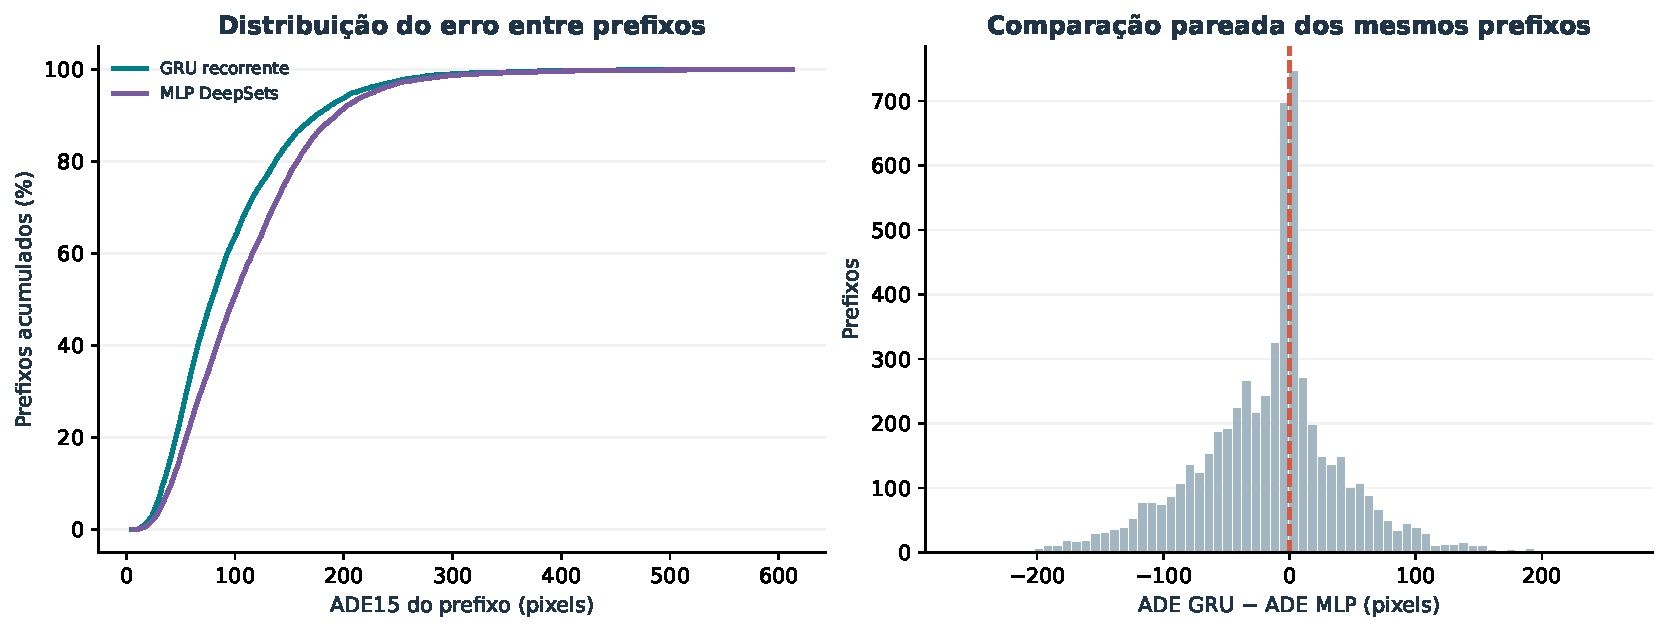
\includegraphics[width=\linewidth,height=.58\textheight,keepaspectratio]{../figures/05_paired_errors.pdf}\caption{Distribuição dos erros e diferenças GRU-MLP sobre os mesmos IDs/cortes16/32 em k=15. Valores negativos favorecem a GRU; valores positivos favorecem a MLP. Nenhum prefixo foi escolhido por seu acerto.}\end{figure}
\section{Quantidade de contexto e previsão progressiva}
A evolução com prefixos de 8/16/32/64 eventos é uma análise de previsão progressiva, não de reconhecimento da categoria. Ao mudar o instante de origem, também se mudam os eventos futuros a prever; a figura informa as coortes disponíveis. Por isso, uma curva melhor não prova isoladamente que mais passado foi a causa. A análise complementar fixa origem 64 e futuro 15, variando somente a janela disponível. Nessa análise, janelas internas diferem dos prefixos de início vistos no treino e são tratadas como sensibilidade fora da distribuição de treinamento, sem retreino.
\begingroup\small\setlength{\tabcolsep}{4pt}\begin{longtable}{lrrrr}
\caption{Sensibilidade à janela com origem 64 e os mesmos alvos15.}\\
\toprule
Rede & Janela & Prefixos & ADE & FDE \\ 
\midrule\endfirsthead
\toprule
Rede & Janela & Prefixos & ADE & FDE \\ 
\midrule\endhead
\bottomrule\endfoot
GRU & 8 & 240 & 138,3 & 225,2 \\
MLP DeepSets & 8 & 240 & 134,0 & 220,8 \\
GRU & 16 & 240 & 131,8 & 223,8 \\
MLP DeepSets & 16 & 240 & 131,6 & 215,5 \\
GRU & 32 & 240 & 121,5 & 200,8 \\
MLP DeepSets & 32 & 240 & 130,4 & 221,1 \\
GRU & 64 & 240 & 105,3 & 169,0 \\
MLP DeepSets & 64 & 240 & 126,2 & 213,1 \\
\end{longtable}\endgroup
\begin{figure}[H]\centering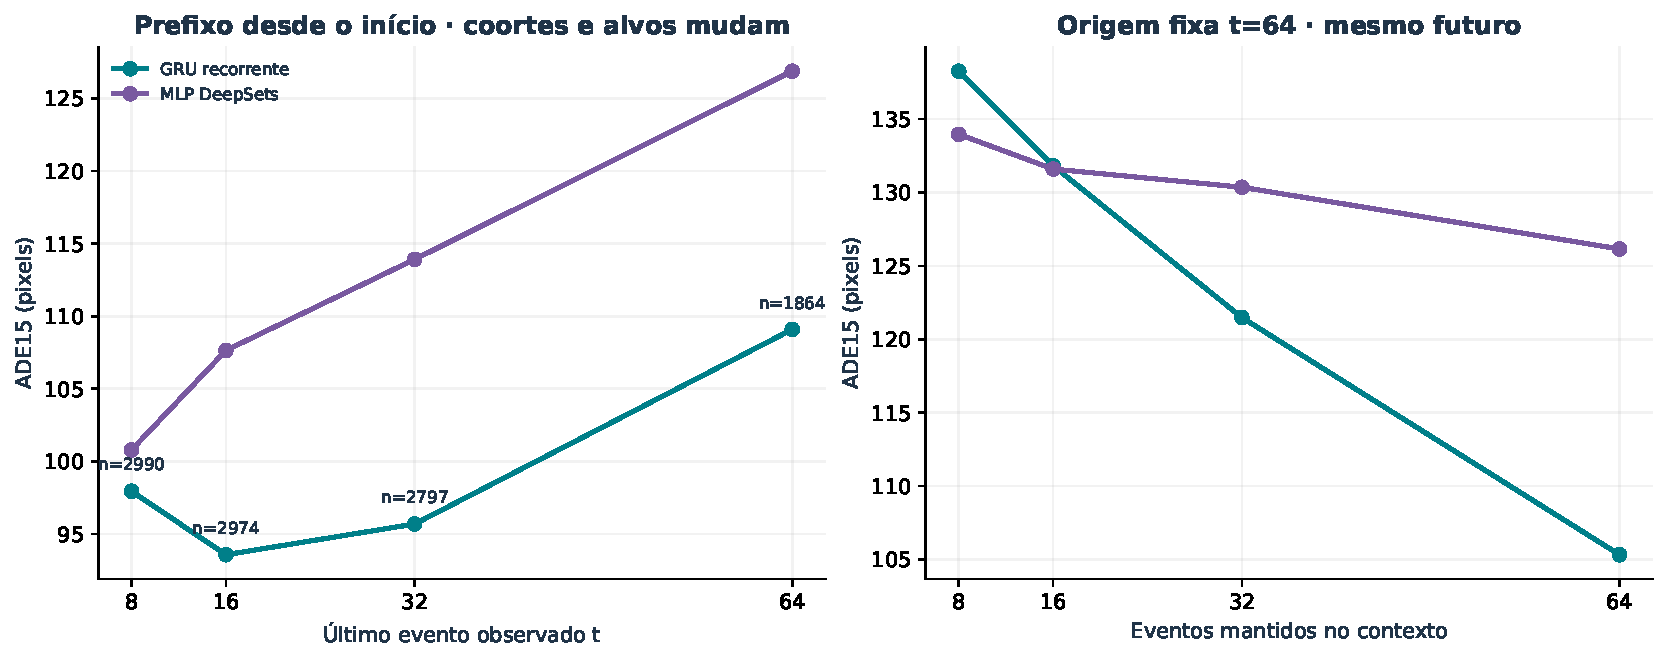
\includegraphics[width=\linewidth,height=.58\textheight,keepaspectratio]{../figures/02_prefix_cohorts.pdf}\caption{À esquerda, prefixos8/16/32/64 desde o início: coortes e alvos mudam, portanto não é uma ablação causal de contexto. À direita, origem fixa64 e alvos comuns, variando apenas a janela observada. Essas janelas internas não eram origens de treino; é análise de sensibilidade com coorte fixa de desenhos longos.}\end{figure}
\section{Cruzamentos, sobreposição e estados de caneta}
Cruzamentos do prefixo e frequência de pen-up são descritores calculados antes do futuro, comuns às duas redes. A comparação condicionada ajuda a verificar se certos padrões são mais difíceis ou favorecem um encoder. Ela não identifica causalidade: complexidade, tamanho e categoria também variam entre grupos. O comparador é um MLP de eventos, não uma CNN de imagem; não se avaliou diretamente a alegação de que a RNN seria imune ao borrão de uma imagem raster. O estado de caneta fornece separações observadas, mas não garante que a rede saiba qual segmento é olho, rosto ou contorno.
\begingroup\small\setlength{\tabcolsep}{4pt}\begin{longtable}{lrrrr}
\caption{Diferenças condicionadas em k15, seed42; valores negativos favorecem a GRU.}\\
\toprule
Descritor & Grupo & Prefixos & Diferença & IC95 \\ 
\midrule\endfirsthead
\toprule
Descritor & Grupo & Prefixos & Diferença & IC95 \\ 
\midrule\endhead
\bottomrule\endfoot
Cruzamentos & 0 & 2.316 & -17,94 & [-20,27; -15,38] \\
Cruzamentos & 1 & 353 & -22,48 & [-28,39; -16,27] \\
Cruzamentos & $\geq$2 & 128 & -11,90 & [-20,32; -4,04] \\
Pen-up & 0 & 1.428 & -15,71 & [-18,89; -12,08] \\
Pen-up & 1–2 & 1.203 & -23,02 & [-26,58; -19,61] \\
Pen-up & $\geq$3 & 166 & -5,39 & [-12,10; 1,38] \\
\end{longtable}\endgroup
\begin{figure}[H]\centering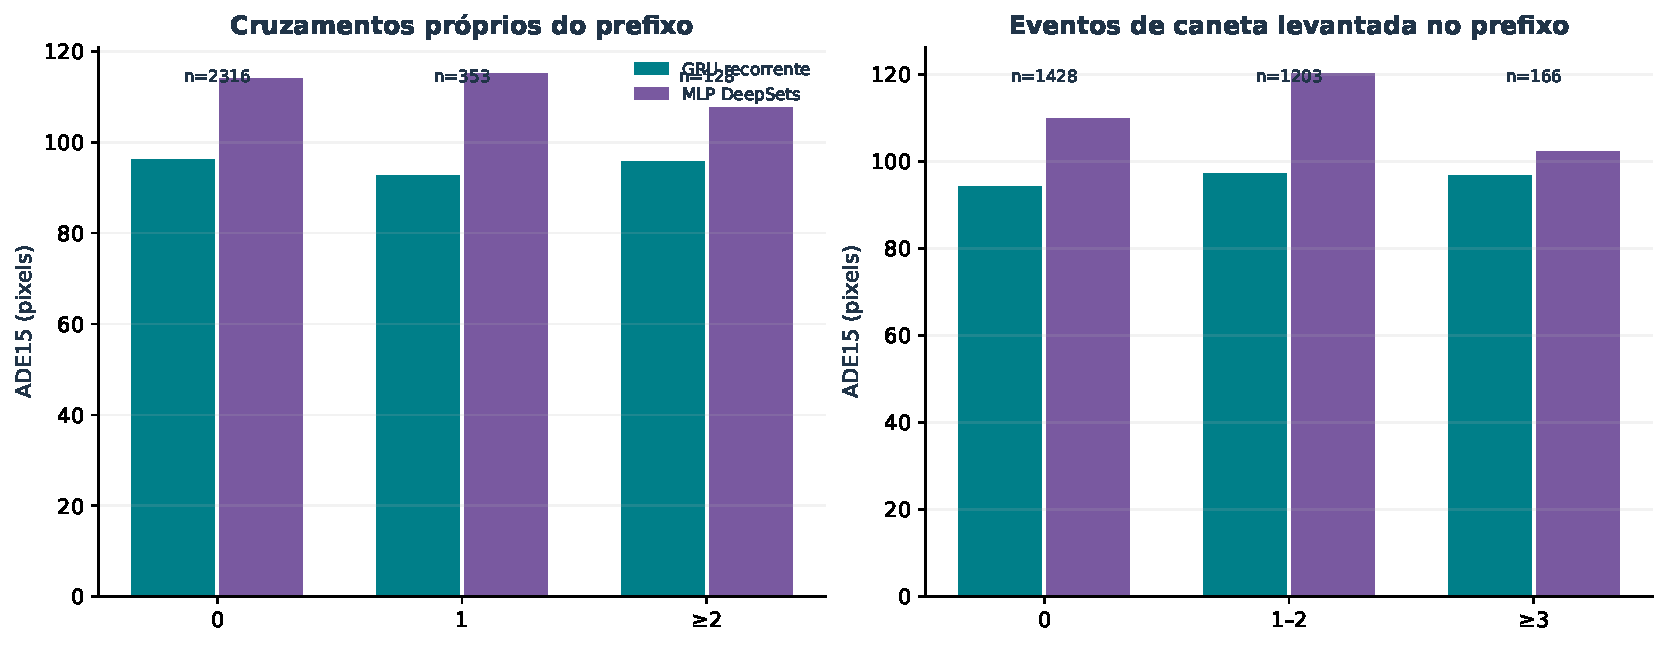
\includegraphics[width=\linewidth,height=.58\textheight,keepaspectratio]{../figures/03_geometry_groups.pdf}\caption{Erro de previsão condicionado a descritores do passado, t=32 e k=15. Cruzamentos são interseções próprias entre segmentos de tinta não adjacentes; extremos compartilhados e sobreposições colineares não são contados. Classes e estilos podem ter distribuições diferentes entre grupos. Não é demonstração de imunidade a borrões ou sobreposição visual.}\end{figure}
\section{Ordem, posição, escala e pausas: controles de sensibilidade}
A translação das coordenadas desaparece na codificação por deslocamentos e posições relativas; esse controle deve beneficiar ambos os modelos, e não ser atribuído à recorrência. Já $\Delta$x/$\Delta$y preservam magnitude: uma casa maior gera deslocamentos maiores. Portanto, não há independência automática de escala. Avaliamos fatores 0,75/1,25 e ADE dividido pelo fator para comparar a escala do erro. A permutação mantém o primeiro evento e um sufixo suficiente para preservar os últimos três segmentos válidos e o referencial do decoder. Permutar vetores já codificados pode produzir uma sequência fisicamente inconsistente; o teste mede sensibilidade do encoder, não uma intervenção causal válida no desenho. Retirar canais de caneta ou relógio sem retreino também é uma perturbação fora da distribuição. No ensaio de pen-up, mantemos explicitamente o quadro original do decoder para não misturar mudança de representação geométrica com a retirada do canal.
\begingroup\small\setlength{\tabcolsep}{4pt}\begin{longtable}{lrrrrr}
\caption{Sensibilidades em k15 na subamostra determinística; não são novos modelos retreinados.}\\
\toprule
Rede & Cenário & n & ADE & ADE/escala & Razão/base \\ 
\midrule\endfirsthead
\toprule
Rede & Cenário & n & ADE & ADE/escala & Razão/base \\ 
\midrule\endhead
\bottomrule\endfoot
GRU & Original & 240 & 95,5 & 95,5 & 1,00 \\
GRU & Translação & 240 & 95,5 & 95,5 & 1,00 \\
GRU & Escala 0,75 & 240 & 79,6 & 106,2 & 1,11 \\
GRU & Escala 1,25 & 240 & 116,2 & 93,0 & 0,97 \\
GRU & Ordem permutada & 240 & 111,7 & 111,7 & 1,17 \\
GRU & Sem pen-up & 240 & 95,7 & 95,7 & 1,00 \\
GRU & Sem tempo & 240 & 100,9 & 100,9 & 1,06 \\
MLP DeepSets & Original & 240 & 119,8 & 119,8 & 1,00 \\
MLP DeepSets & Translação & 240 & 119,8 & 119,8 & 1,00 \\
MLP DeepSets & Escala 0,75 & 240 & 102,4 & 136,5 & 1,14 \\
MLP DeepSets & Escala 1,25 & 240 & 146,1 & 116,9 & 0,98 \\
MLP DeepSets & Ordem permutada & 240 & 119,8 & 119,8 & 1,00 \\
MLP DeepSets & Sem pen-up & 240 & 121,4 & 121,4 & 1,01 \\
MLP DeepSets & Sem tempo & 240 & 125,6 & 125,6 & 1,05 \\
\end{longtable}\endgroup
\begin{figure}[H]\centering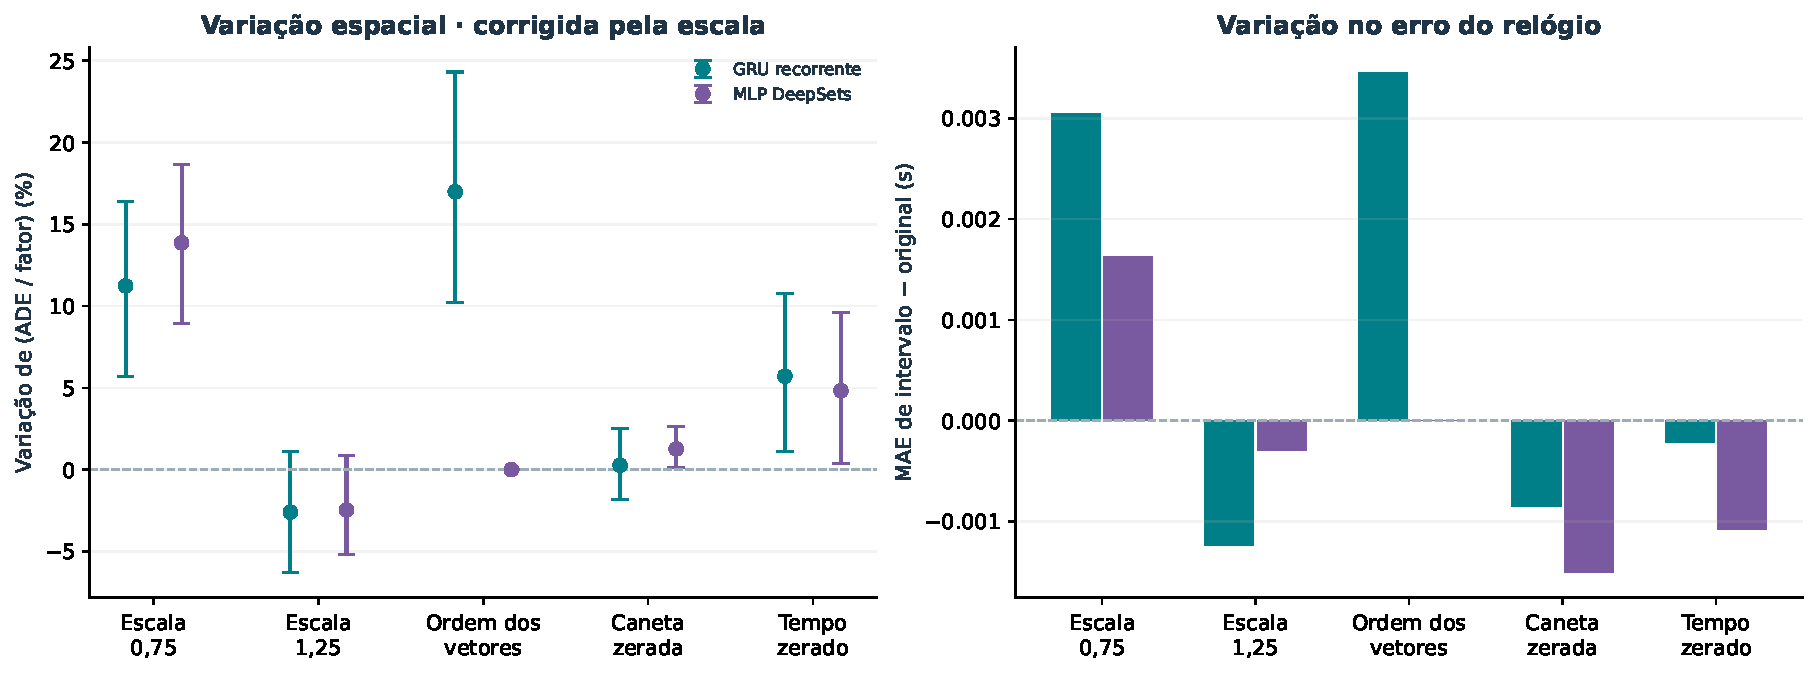
\includegraphics[width=\linewidth,height=.58\textheight,keepaspectratio]{../figures/04_sensitivities.pdf}\caption{Intervenções sintéticas na entrada, sem retreino, t=32 e k=15. O erro espacial é dividido pelo fator de escala antes de comparar, evitando confundir aumento geométrico com perda de consistência. A ordem permuta vetores prontos e pode produzir sequências não físicas. Caneta zerada usa quadro geométrico original congelado; tempo zerado significa intervalos nulos, não informação ausente.}\end{figure}
\begin{figure}[H]\centering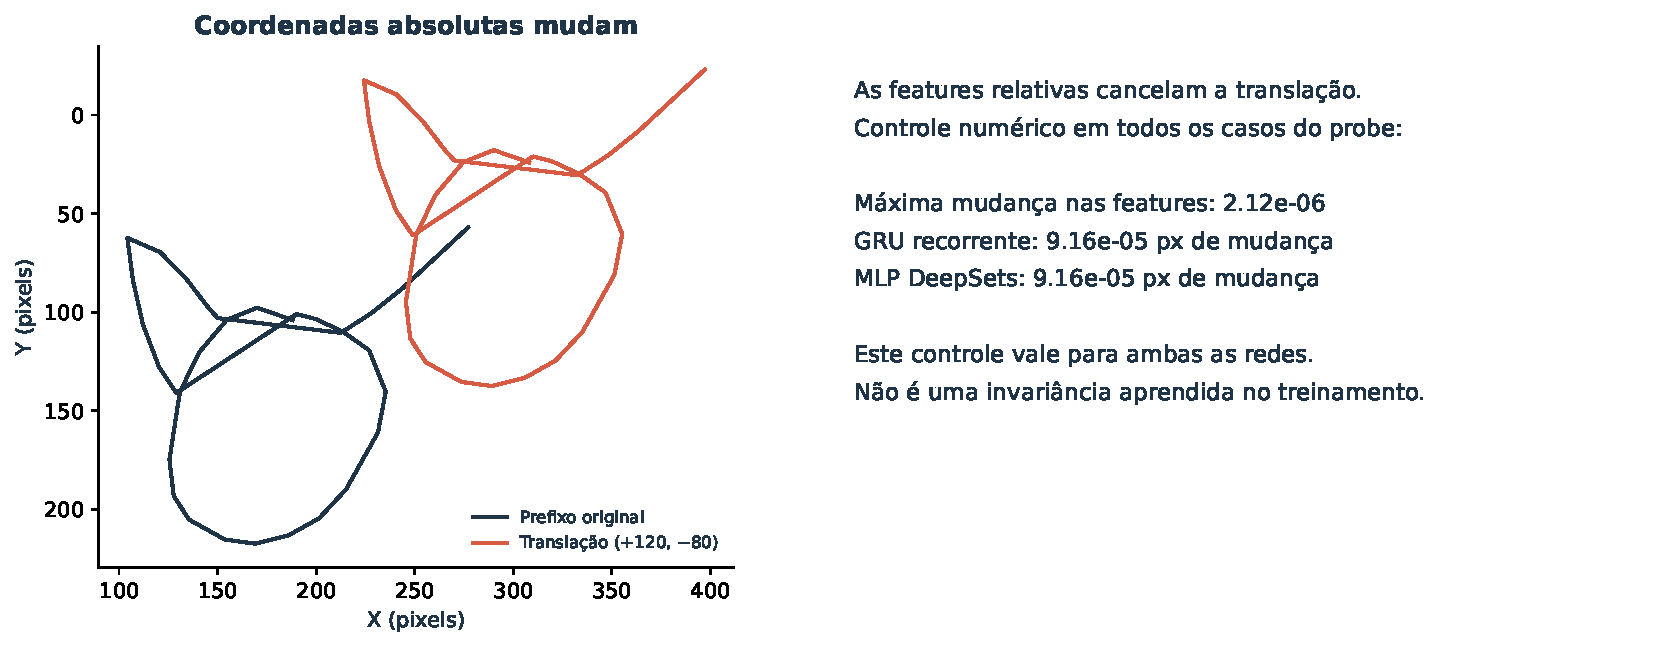
\includegraphics[width=\linewidth,height=.58\textheight,keepaspectratio]{../figures/07_translation_control.pdf}\caption{Controle de pré-processamento. Transladar todas as coordenadas por um deslocamento comum cancela nas features relativas; isso beneficia ambas as arquiteturas. Os resíduos numéricos são reportados sem atribuir a invariância ao treinamento.}\end{figure}
\subsection{O que os controles efetivamente mostraram}
Na subamostra de 240 prefixos, mudar a ordem interna aumentou o ADE da GRU em 17,0\%, enquanto o MLP permaneceu numericamente igual (razão 1,0000). O referencial do decoder não mudou (diferença máxima 0,000000). A GRU trocou o modo escolhido em 59,6\% dos prefixos. Isso confirma sensibilidade da representação recorrente à ordenação, mas não torna a permutação uma trajetória humana válida. Na translação, a maior alteração de previsão foi 0,000092 pixel; a estabilidade resulta do pré-processamento comum. Zerar o relógio aumentou o ADE em 5,7\% na GRU e 4,8\% no MLP: o canal temporal ajuda as duas arquiteturas. Os fatores de escala não produziram invariância exata. Na análise com origem64, o ADE da GRU passou de 138,3 para 105,3 pixels ao ampliar a janela de8para64eventos; o MLP passou de 134,0 para 126,2. Os ensaios com janelas internas são fora da distribuição de início de desenho; são sensibilidades, não garantias de robustez.
\section{Tempo e separação de traços}
F1 de pen-up complementa os erros espaciais porque a maioria dos eventos mantém a caneta no papel. Uma linha próxima em pixels pode ligar regiões que deveriam estar separadas. O modelo estima intervalos positivos enquanto ativo e zero após encerramento. Comparamos o MAE do intervalo à referência que repete a mediana positiva do prefixo. A regra absorvente de encerramento mantém a posição para que terminar antes da hora continue contando como erro. Melhorar ADE não implica melhorar relógio ou F1; esses aspectos são reportados separadamente. Os valores baixos de F1 mostram que as redes ainda erram separações de traços, contrariando a hipótese de compreensão perfeita dos componentes de um objeto.
\begingroup\small\setlength{\tabcolsep}{4pt}\begin{longtable}{lrrrrr}
\caption{Caneta e relógio; médias de três seeds. MAE em segundos por intervalo.}\\
\toprule
k & Rede & F1 pen-up & Fim precoce (\%) & MAE dt & Mediana dt \\ 
\midrule\endfirsthead
\toprule
k & Rede & F1 pen-up & Fim precoce (\%) & MAE dt & Mediana dt \\ 
\midrule\endhead
\bottomrule\endfoot
5 & GRU & 0,131 & 0,0 & 0,059 & 0,055 \\
5 & MLP DeepSets & 0,080 & 0,0 & 0,061 & 0,055 \\
15 & GRU & 0,109 & 0,2 & 0,061 & 0,056 \\
15 & MLP DeepSets & 0,083 & 0,1 & 0,063 & 0,056 \\
30 & GRU & 0,115 & 4,2 & 0,062 & 0,057 \\
30 & MLP DeepSets & 0,092 & 4,3 & 0,063 & 0,057 \\
\end{longtable}\endgroup
\begin{figure}[H]\centering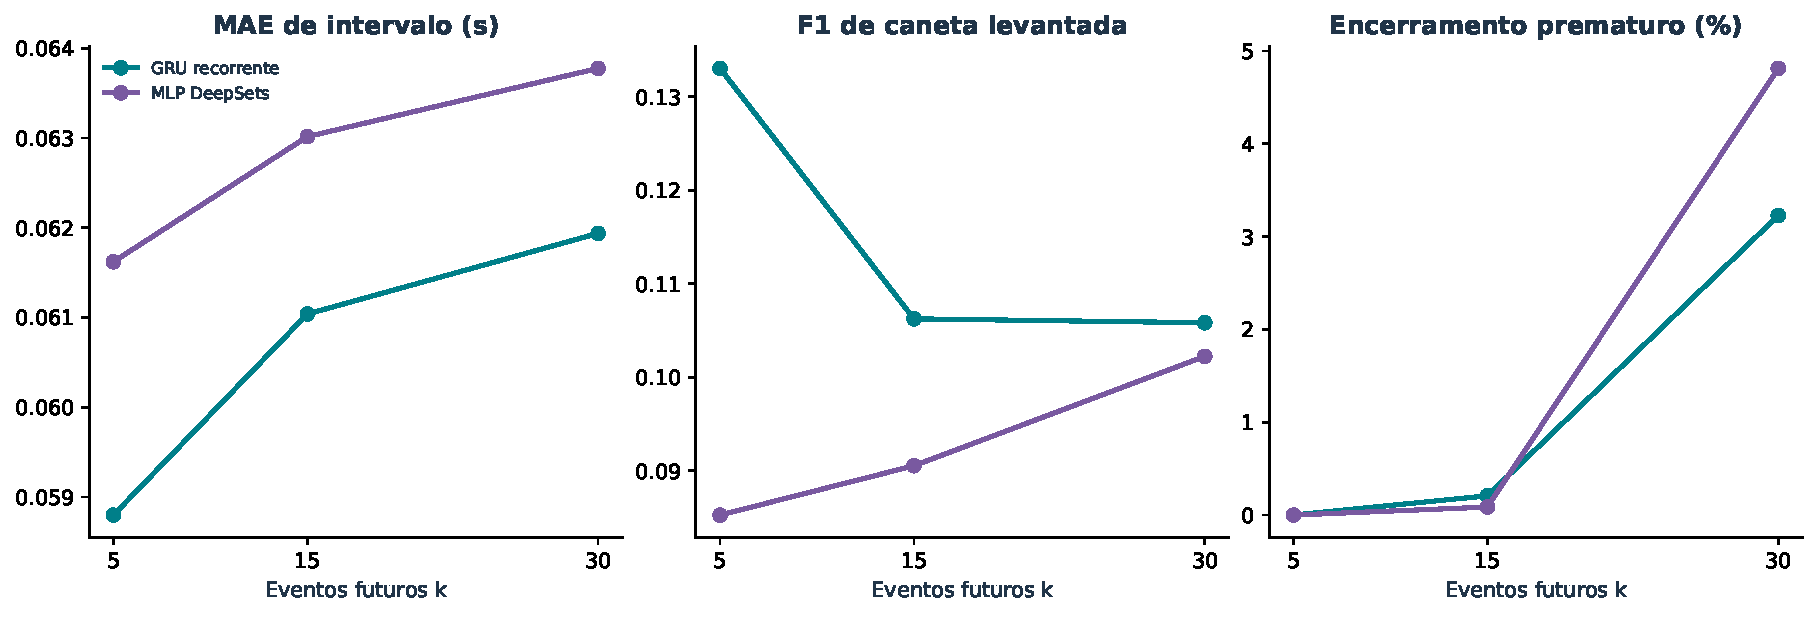
\includegraphics[width=\linewidth,height=.58\textheight,keepaspectratio]{../figures/09_time_pen_quality.pdf}\caption{Previsão temporal e de estado, execução42 nos cortes16/32. F1 é da classe pen-up; encerramento prematuro ocorre quando a rede encerra antes dos eventos futuros disponíveis. Acurácia total da caneta não é usada para ocultar desequilíbrio.}\end{figure}
\section{Casos visuais e diferenças entre categorias}
Os exemplos da demonstração são escolhidos na validação por regras documentadas: categorias, disponibilidade de futuro e casos em que cada rede apresenta menor erro. Esse critério produz exemplos explicativos, e não uma amostra aleatória para estimar vantagem média. O relatório inclui vitórias do MLP e falhas da GRU. O futuro real serve à visualização e às métricas, sem entrar na inferência. As curvas X/Y e o desenho 2D representam a mesma previsão; no painel temporal mostramos parte do passado para legibilidade, embora o modelo receba todo o prefixo indicado.
\begin{figure}[H]\centering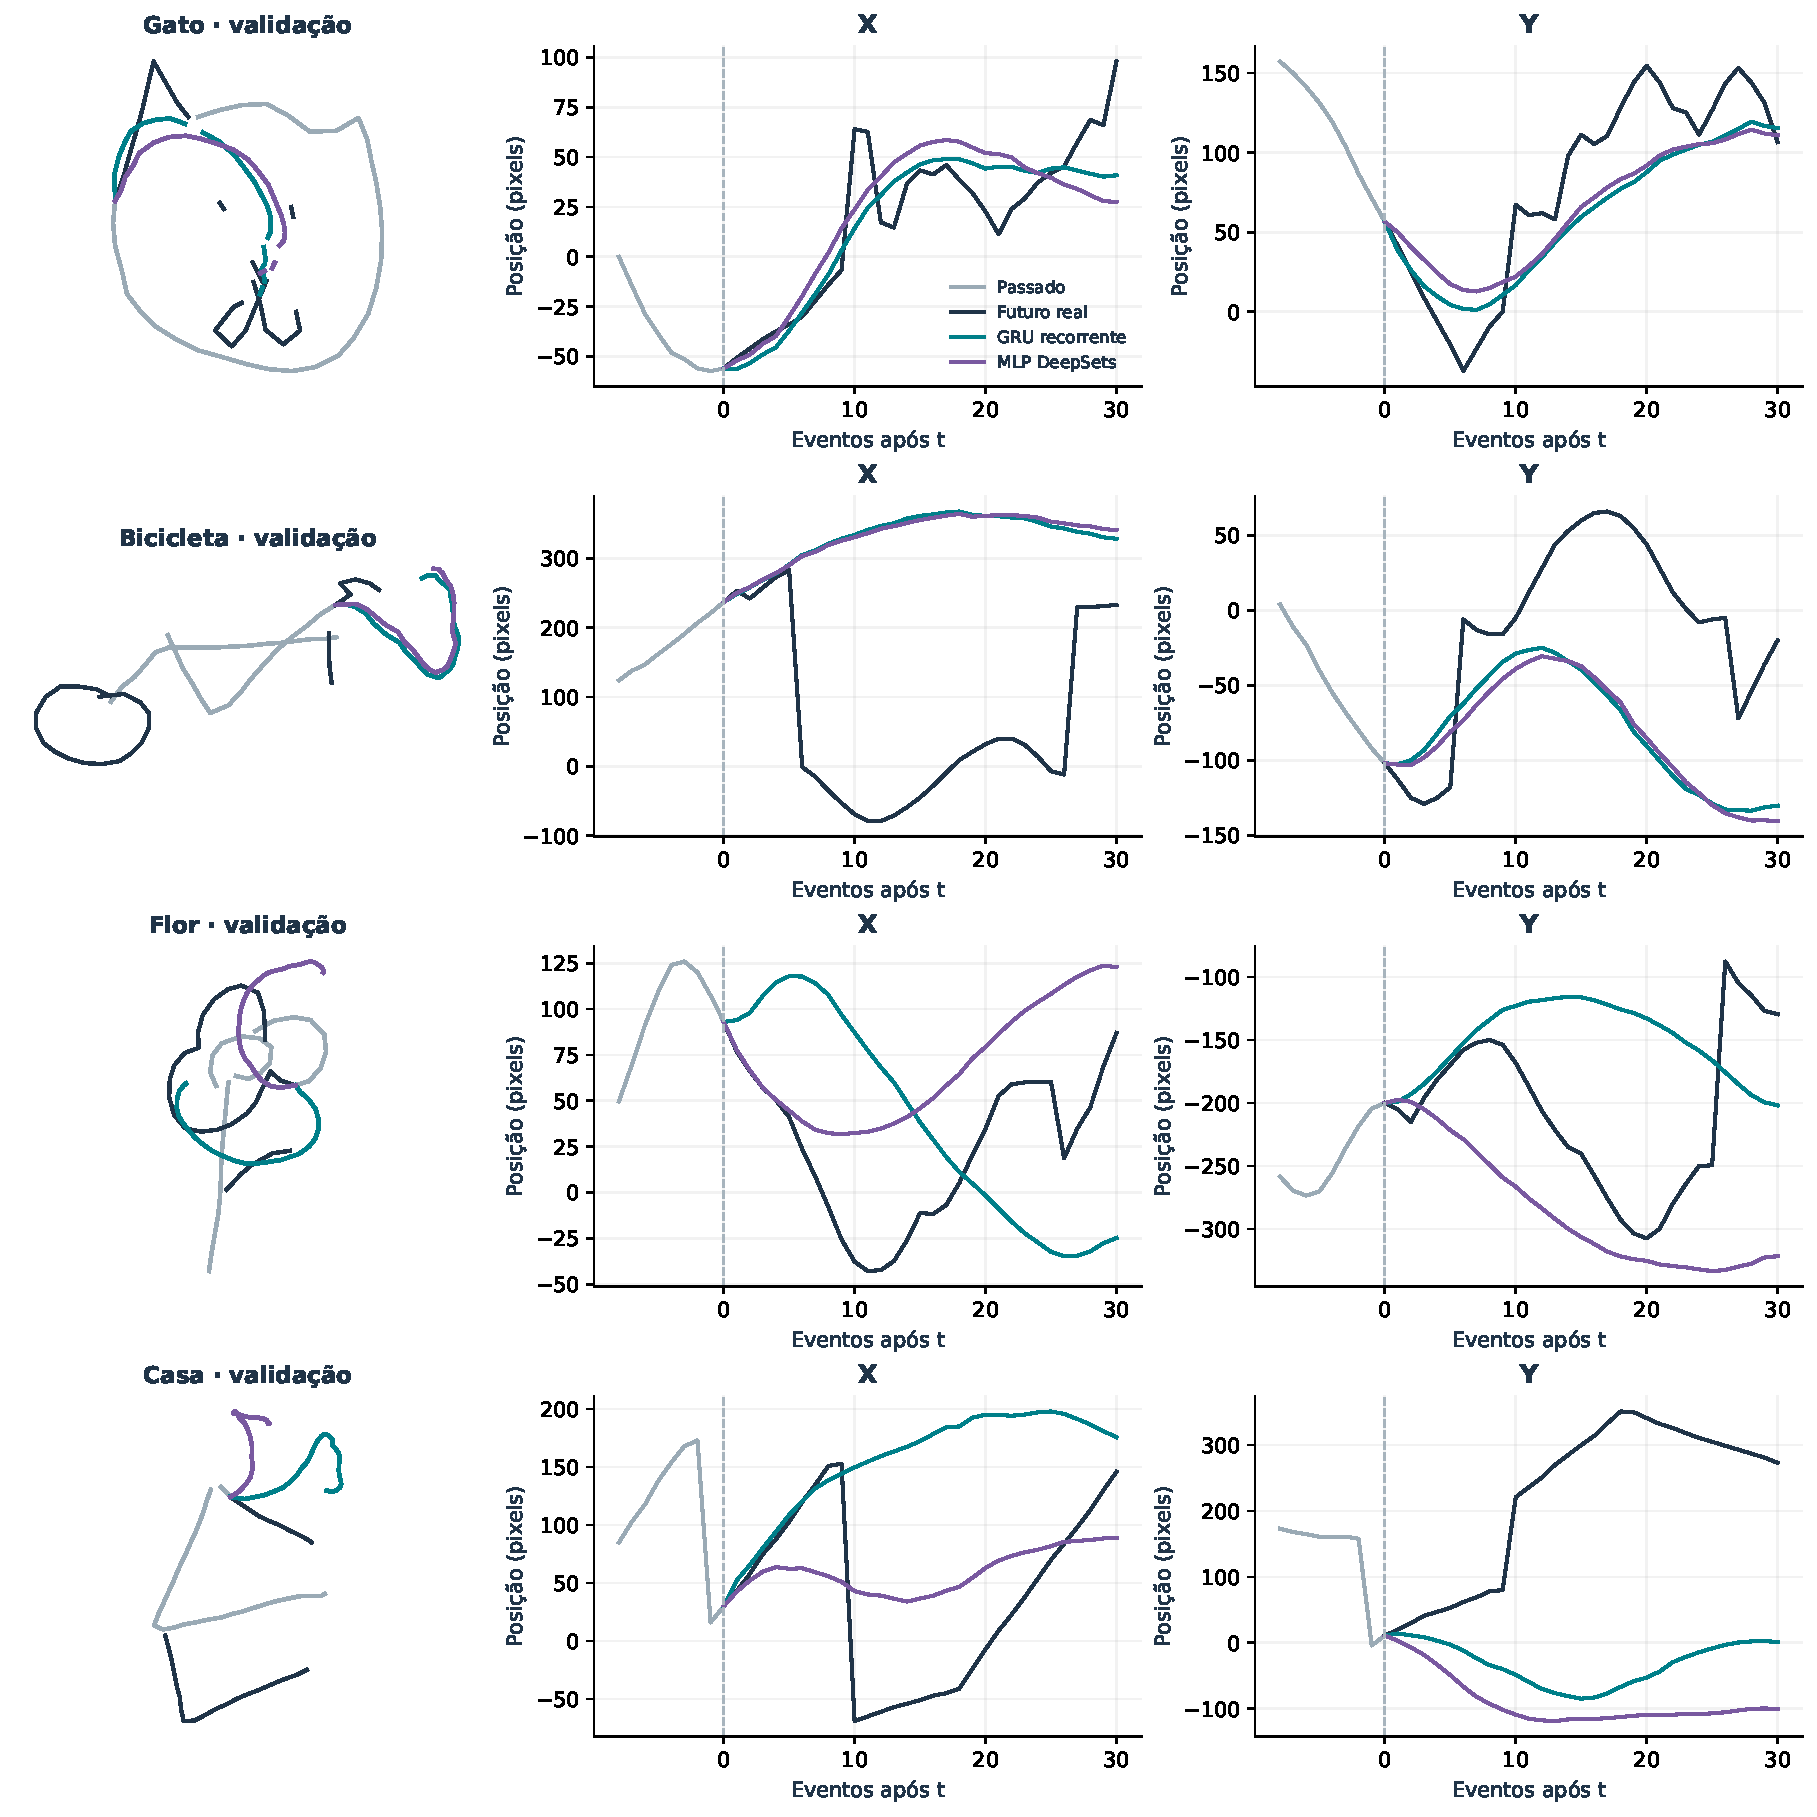
\includegraphics[width=\linewidth,height=.58\textheight,keepaspectratio]{../figures/06_examples_2d_xy.pdf}\caption{Casos de validação: primeiras ocorrências elegíveis por regras declaradas, incluindo previsões próximas e vitórias de cada rede quando disponíveis. Não são os melhores acertos do teste. A representação2D usa o prefixo32 completo; X/Y mostram os últimos9 observados e os30 futuros. Categoria verdadeira fornecida.}\end{figure}
\begin{figure}[H]\centering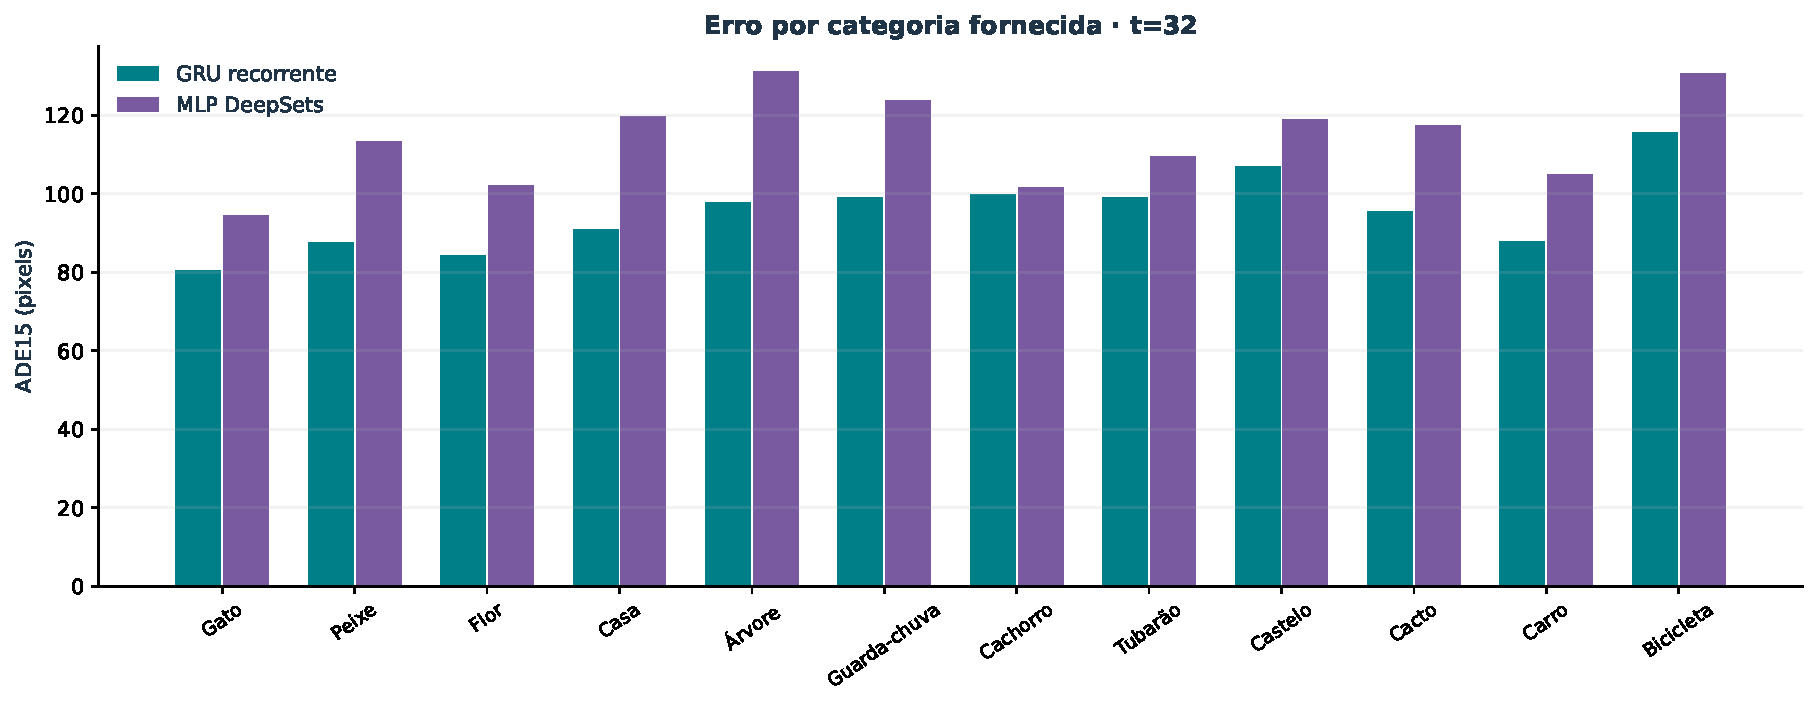
\includegraphics[width=\linewidth,height=.58\textheight,keepaspectratio]{../figures/08_category_comparison.pdf}\caption{Erro de previsão em15 eventos, origem32, separado pela categoria fornecida ao modelo. Não é acurácia de reconhecimento; as duas redes recebem a mesma condição de categoria e os mesmos desenhos.}\end{figure}
\section{Software de demonstração e reprodução}
O site permite escolher uma categoria fornecida, revelar o prefixo de um exemplo real, selecionar horizonte, comparar a GRU com o MLP, avançar pontos lentamente e exibir o futuro real para conferência. A categoria é informada explicitamente: não há reconhecedor embutido no experimento. O usuário também pode desenhar e solicitar previsões locais, sem enviar o desenho a um servidor. O ritmo da reprodução serve à apresentação e não altera timestamps. Controles de ordem, escala e posição devem ser lidos como experimentos de sensibilidade, não como garantias de robustez. Os pesos executados no navegador são confrontados numericamente com PyTorch. O repositório projeto4-irn contém código, dados preparados com proveniência, configs, históricos, métricas, figuras e este único relatório. A publicação usa GitHub Pages e não precisa de backend de treinamento.
\section{Limitações e conclusão}
A comparação testa uma GRU concreta contra um MLP DeepSets concreto com decoder comum. Não demonstra vantagem sobre qualquer rede, nem mede reconhecimento de objetos. O banco de modos e a categoria fornecida restringem as continuações; o mesmo passado pode admitir vários futuros humanos válidos. A busca tem orçamento finito, duas seeds na decisão e três na avaliação; não assegura arquitetura ótima. O teste previamente explorado e a ausência de separação por autor limitam validade externa. Os controles diferenciam benefícios da representação, da recorrência e do decoder. A conclusão deve considerar em conjunto erro espacial, caneta, tempo, grupos de desenhos e exemplos em que cada rede falha, sem transformar memória recorrente em uma promessa de perfeição.
\section*{Referências}\begin{enumerate}
\item \href{https://github.com/googlecreativelab/quickdraw-dataset}{Google Quick, Draw! Dataset — vetores, timestamps e licença.}
\item \href{https://arxiv.org/abs/1406.1078}{Cho et al. (2014) — unidades recorrentes com portas.}
\item \href{https://arxiv.org/abs/1703.06114}{Zaheer et al. (2017) — Deep Sets e agregação invariante a permutações.}
\item \href{https://proceedings.mlr.press/v100/chai20a.html}{Chai et al. (2020) — MultiPath, inspiração para modos de trajetória.}
\item \href{https://arxiv.org/abs/1704.03477}{Ha e Eck (2017) — A Neural Representation of Sketch Drawings.}
\end{enumerate}\small Dados: Google Quick, Draw!, CC BY 4.0. Código e redação elaborados com auxílio de IA; revisar antes da entrega acadêmica.\end{document}